% Build twice here: pdflatex -interaction=nonstopmode -halt-on-error resume7An26w.tex
\documentclass[a4paper,10pt,pdflatex,ja=standard,jafont=ipaex-type1,
  magstyle=real,scale=1]{bxjsarticle}
\usepackage{lmodern}
\usepackage{amsmath,amssymb,mathtools}
\usepackage{geometry}
\geometry{reset,left=22mm,right=22mm,top=20mm,bottom=17mm,
  headheight=13pt,headsep=6mm,footskip=10mm}
\usepackage{xcolor}
\usepackage{enumitem}
\usepackage{array,booktabs,tabularx}
\usepackage{fancyhdr}
\usepackage{lastpage}
\usepackage{tikz}
\usetikzlibrary{arrows.meta,calc,decorations.pathreplacing}

\definecolor{ink}{HTML}{193A5C}
\definecolor{accent}{HTML}{237D82}
\definecolor{soft}{HTML}{EAF3F3}
\definecolor{muted}{HTML}{52616B}
\newcommand{\coursename}{解析学 II}
\newcommand{\handoutnumber}{7}
\pagestyle{fancy}
\fancyhf{}
\fancyhead[L]{\small\color{ink}\coursename{}・授業要約と演習}
\fancyhead[R]{\small\color{ink}第\handoutnumber 回}
\fancyfoot[C]{\small\color{ink}\thepage/\pageref{LastPage}}
\renewcommand{\headrulewidth}{0.3pt}
\setlength{\parindent}{0pt}
\setlength{\parskip}{2pt}
\setlength{\abovedisplayskip}{5pt}
\setlength{\belowdisplayskip}{5pt}
\setlength{\abovedisplayshortskip}{3pt}
\setlength{\belowdisplayshortskip}{4pt}
\setlist[itemize]{leftmargin=1.8em,itemsep=1pt,topsep=2pt,parsep=0pt}

\newcommand{\handouttitle}[1]{%
  \begin{center}
    {\Large\color{ink}#1}\par\vspace{3mm}
    {\color{accent}\rule{0.88\linewidth}{0.7pt}}
  \end{center}\vspace{-2mm}}
\newcommand{\handout}[2]{%
  \renewcommand{\handoutnumber}{#1}%
  \handouttitle{第#1回\quad #2}}
\newcommand{\topic}[1]{\par\vspace{5pt}%
  {\large\sffamily\mdseries\color{accent}#1}\par\vspace{2pt}}
\newcommand{\keybox}[1]{\par\vspace{3pt}\begingroup
  \setlength{\fboxsep}{4pt}%
  \colorbox{soft}{\parbox{\dimexpr\linewidth-2\fboxsep\relax}{\small #1}}%
  \endgroup\par\vspace{2pt}}
\newenvironment{problems}
  {\begin{enumerate}[leftmargin=2em,itemsep=3pt,topsep=3pt,parsep=0pt,
    font=\color{accent}]}
  {\end{enumerate}}


\newcommand{\examplelabel}[1]{{\sffamily\mdseries\color{ink}#1}}
\newcommand{\problemspace}{\par\vspace{5mm}}
\newcommand{\exercises}{%
  {\color{accent}\hrule height 0.7pt}\vspace{3pt}%
  \topic{演習問題（6題）}%
  {\small 領域と積分範囲を確認し、計算過程も書こう。図を描くと範囲を読み取りやすい。}\par}
\tikzset{
  handout diagram/.style={>={Stealth[length=3.2pt,width=3.2pt]},line join=round,
    every node/.style={font=\scriptsize,text=ink}},
  region/.style={fill=soft,draw=accent,semithick},
  slice/.style={accent,line width=1.8pt},
  guide/.style={muted,densely dashed,thin},
  axis/.style={->,ink,thin}}


% Review Q&A can also be used for actual student feedback when it is available.
\newcommand{\feedback}[2]{%
  \par\addvspace{8pt}\noindent\begin{minipage}{\linewidth}%
  {\color{ink}Q. #1}\par\vspace{2pt}%
  {\color{accent}A. }#2%
  \end{minipage}\par}

\begin{document}
\fontsize{10pt}{13.5pt}\selectfont
\setlength{\abovedisplayskip}{4pt}
\setlength{\belowdisplayskip}{4pt}
% Feedback section: add comments and responses here when available.
\fancyhead[L]{\small\color{ink}\coursename{}・フィードバック}
\handout{7}{前回のコメントへのフィードバック}
% \feedback{comment}{response}
\clearpage

% Previous small-test section: add the questions and solutions here.
\fancyhead[L]{\small\color{ink}\coursename{}・小テスト}
\fancyhead[R]{\small\color{ink}第6回}
\handouttitle{第6回\quad 小テスト}
% Questions and solutions are intentionally blank.
\clearpage

\fancyhead[L]{\small\color{ink}\coursename{}・授業要約と演習}
\fancyhead[R]{\small\color{ink}第\handoutnumber 回}
\handout{7}{重積分の応用：体積と質量}\label{lesson-start}
\keybox{到達目標：立体の投影領域と上下の境界から積分を設定し、体積・質量・重心を求められる。
密度の変化と座標変換の両方を積分式に反映しよう。}

\topic{上下のグラフに挟まれた立体の体積}
$D\subset\mathbb R^2$ を有界な積分可能領域、$\phi,\psi$ を $D$ 上の連続関数、$\phi\le\psi$ とし
$$
 V=\{(x,y,z):(x,y)\in D,\ \phi(x,y)\le z\le\psi(x,y)\}
$$
とする。各点の柱の高さは $\psi-\phi$ なので
$$
 \operatorname{Vol}(V)=\iint_D(\psi-\phi)\,dx\,dy
 =\iiint_V1\,dx\,dy\,dz.
$$
上面と下面を入れ替えず、投影領域 $D$ と高さの範囲を先に決める。


\par\vspace{2pt}\noindent
\begin{minipage}[b]{0.48\linewidth}\centering
\begin{tikzpicture}[handout diagram,x=1cm,y=0.8cm]
\path[region] (0,0.5) -- (3,0.85) -- (3,2.55) -- (0,2) -- cycle;
 \draw[accent] (0,2) .. controls (1,2.25) and (2,2.35) .. (3,2.55);
 \draw[slice,<->] (1.6,0.72) -- (1.6,2.3);
 \node[right] at (1.7,1.5) {$\psi-\phi$};
 \draw[guide] (1.6,0) -- (1.6,0.72);
 \draw[axis] (0,0) -- (3.6,0) node[right] {底面の位置};
 \draw[axis] (0,0) -- (0,3) node[above] {$z$};
 \node[above] at (2.7,2.55) {$z=\psi$};
 \node[below] at (2.7,0.8) {$z=\phi$};
\end{tikzpicture}\par
{\small\color{muted}柱の高さは「上面 $-$ 下面」（断面の模式図）}\par
\end{minipage}\hfill
\begin{minipage}[b]{0.48\linewidth}\centering
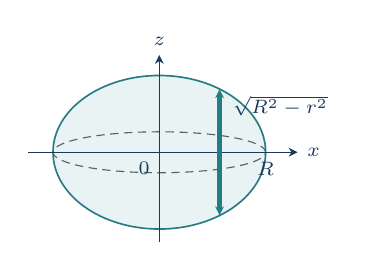
\begin{tikzpicture}[handout diagram,x=0.9cm,y=0.65cm]
\path[region] (0,0) circle (1.5);
 \draw[guide] (0,0) ellipse (1.5 and 0.4);
 \draw[axis] (-1.85,0) -- (1.95,0) node[right] {$x$};
 \draw[axis] (0,-1.75) -- (0,1.9) node[above] {$z$};
 \draw[slice,<->] (0.85,-1.23) -- (0.85,1.23);
 \node[right] at (0.9,0.9) {$\sqrt{R^2-r^2}$};
 \node[below left] at (0,0) {$0$};
 \node[below] at (1.5,0) {$R$};
\end{tikzpicture}\par
{\small\color{muted}断面 $y=0$：$r=|x|$、縦の長さは $2\sqrt{R^2-r^2}$}\par
\end{minipage}
\par\vspace{2pt}

\topic{例：半径 $R>0$ の球の体積}
$D=\{(x,y):x^2+y^2\le R^2\}$ の上で
$\psi=\sqrt{R^2-x^2-y^2}$、$\phi=-\psi$ とすると
$$
 \begin{aligned}
 \operatorname{Vol}(V)
 &=\int_0^{2\pi}\int_0^R2\sqrt{R^2-r^2}\,r\,dr\,d\theta\\
 &=4\pi\left[-\frac13(R^2-r^2)^{3/2}\right]_0^R
 =\frac{4\pi R^3}{3}.
 \end{aligned}
$$


\topic{密度を積分して総量を求める}
質量密度 $\rho\ge0$ が与えられ、$\rho$ が $V$ 上可積分なら、質量は
$$
 M=\iiint_V\rho(x,y,z)\,dx\,dy\,dz
 =\iint_D\left(\int_{\phi(x,y)}^{\psi(x,y)}\rho(x,y,z)\,dz\right)dx\,dy.
$$
密度が一定 $\rho_0$ なら $M=\rho_0\operatorname{Vol}(V)$。
電荷密度・エネルギー密度を積分すれば、それぞれ全電荷・全エネルギーになる。


\par\vspace{2pt}\noindent
\begin{minipage}[b]{0.98\linewidth}\centering
\begin{tikzpicture}[handout diagram,x=0.75cm,y=0.65cm]
\foreach \z/\shade in {0/8,0.45/15,0.9/23,1.35/32}{
  \filldraw[fill=accent!\shade,draw=accent] (0,\z) rectangle (2.6,{\z+0.45});}
 \draw[axis] (-0.4,0) -- (-0.4,2.4) node[above] {$z$};
 \draw[<->,ink] (2.9,0) -- (2.9,1.8) node[midway,right] {$H$};
 \node[right] at (3.4,1.5) {上ほど密度が大きい};
 \node[right] at (3.4,0.6) {各層で $dM=\rho\,dV$};
\end{tikzpicture}\par
{\small\color{muted}密度が変わると、同じ体積でも質量が変わる}\par
\end{minipage}
\par\vspace{2pt}

\newpage
% Keep the remaining summary in the upper half of page 2.
\noindent\begin{minipage}[b][\dimexpr0.5\textheight-\parskip\relax][t]{\linewidth}
\topic{円柱座標と球面座標の体積要素}
円柱座標 $x=r\cos\theta,\ y=r\sin\theta$ では
$$
 dx\,dy\,dz=r\,dr\,d\theta\,dz.
$$
球面座標を $x=s\sin\alpha\cos\theta,\ y=s\sin\alpha\sin\theta,\ z=s\cos\alpha$
（$s\ge0,\ 0\le\alpha\le\pi,\ 0\le\theta<2\pi$）と定めると
$$
 dx\,dy\,dz=s^2\sin\alpha\,ds\,d\alpha\,d\theta.
$$
円柱・球の対称性に合う座標を選ぶと、領域と被積分関数が簡単になる。


\topic{例：円柱の質量と重心}
$V=\{x^2+y^2\le1,\ 0\le z\le2\}$、$\rho=z$ とする。
$$
 M=\int_0^{2\pi}\int_0^1\int_0^2z r\,dz\,dr\,d\theta=2\pi.
$$
一般に $M>0$ の物体の重心は $\overline x=M^{-1}\iiint_Vx\rho\,dV$ などで定まる。
この例では回転対称性から $\overline x=\overline y=0$、また
$$
 \overline z=\frac1{2\pi}\int_0^{2\pi}\int_0^1\int_0^2z^2r\,dz\,dr\,d\theta=\frac43.
$$
\keybox{体積は1を、質量は密度を積分する。座標を変換したら、体積要素のヤコビアンも必ず付ける。}

\par\vspace{2pt}\noindent
\begin{minipage}[b]{0.48\linewidth}\centering
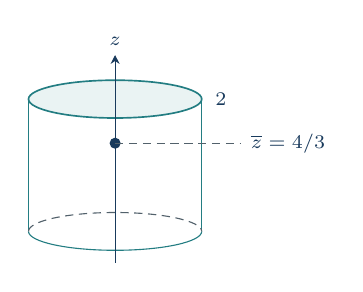
\begin{tikzpicture}[handout diagram,x=1cm,y=0.8cm]
\draw[accent] (-1.1,0) -- (-1.1,2.1) (1.1,0) -- (1.1,2.1);
 \path[region] (0,2.1) ellipse (1.1 and 0.3);
 \draw[accent] (-1.1,0) arc[start angle=180,end angle=360,x radius=1.1,y radius=0.3];
 \draw[guide] (-1.1,0) arc[start angle=180,end angle=0,x radius=1.1,y radius=0.3];
 \draw[axis] (0,-0.5) -- (0,2.8) node[above] {$z$};
 \fill[ink] (0,1.4) circle (2pt);
 \draw[guide] (0,1.4) -- (1.6,1.4) node[right] {$\overline z=4/3$};
 \node[right] at (1.15,2.1) {$2$};
\end{tikzpicture}\par
{\small\color{muted}密度 $\rho=z$ の重心は中央より上}\par
\end{minipage}\hfill
\begin{minipage}[b]{0.48\linewidth}\centering
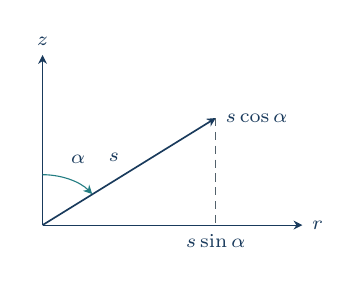
\begin{tikzpicture}[handout diagram,x=1cm,y=0.8cm]
\draw[axis] (0,0) -- (3.3,0) node[right] {$r$};
 \draw[axis] (0,0) -- (0,2.7) node[above] {$z$};
 \draw[->,ink,semithick] (0,0) -- (2.2,1.7) node[midway,above left] {$s$};
 \draw[guide] (2.2,1.7) -- (2.2,0);
 \draw[accent,->] (0,0.8) arc[start angle=90,end angle=38,radius=0.8];
 \node at (0.45,1.05) {$\alpha$};
 \node[below] at (2.2,0) {$s\sin\alpha$};
 \node[right] at (2.2,1.7) {$s\cos\alpha$};
\end{tikzpicture}\par
{\small\color{muted}球面座標の $\alpha$ は $+z$ 軸から測る}\par
\end{minipage}
\par\vspace{2pt}

\end{minipage}\par\nointerlineskip
% Keep the exercises and writing space in the lower half of page 2.
\noindent\begin{minipage}[b][0.5\textheight][t]{\linewidth}
\exercises
\begin{problems}
\item $V=\{(x,y,z):x^2+y^2\le1,\ 0\le z\le1-x^2-y^2\}$ の体積を求めよ。投影領域と上下の境界を明記すること。
\problemspace

\item 半径 $R>0$ の球の体積を球面座標で求め、上下のグラフを用いた計算と一致することを確認せよ。
\problemspace

\item 円柱 $V=\{x^2+y^2\le1,\ 0\le z\le2\}$ に一定密度 $\rho_0>0$ があるときの質量を求めよ。次に密度を $\rho=z$ に変えた場合の質量を求めよ。
\problemspace

\item $V=\{(x,y,z):x,y,z\ge0,\ x+y+z\le1\}$ の体積を累次積分で求めよ。
\problemspace

\item $V=\{(x,y,z):0\le x,y,z\le1\}$、$\rho=1+z$ とする。質量 $M$ と重心の高さ $\overline z$ を求めよ。
\problemspace

\item 半径 $R>0$ の球内で $\rho(x,y,z)=x^2+y^2+z^2$ とする。質量を球面座標で求め、重心が原点となる理由を述べよ。
\problemspace
\end{problems}
\end{minipage}

\newpage
\handouttitle{第7回\quad 演習問題の解答}
{\small 設定した範囲と条件も確認しながら、計算を振り返ろう。}\par
\begin{problems}
\setlength{\itemsep}{7pt}
\item 投影領域は単位円板、下面は $z=0$、上面は $z=1-r^2$。
$$
 \operatorname{Vol}(V)=\int_0^{2\pi}\int_0^1(1-r^2)r\,dr\,d\theta
 =2\pi\left(\frac12-\frac14\right)=\frac\pi2.
$$

\item $0\le s\le R$、$0\le\alpha\le\pi$、$0\le\theta<2\pi$ として
$$
 \operatorname{Vol}(V)
 =\int_0^{2\pi}\int_0^\pi\int_0^R s^2\sin\alpha\,ds\,d\alpha\,d\theta
 =2\pi\cdot2\cdot\frac{R^3}{3}=\frac{4\pi R^3}{3}.
$$
上下のグラフを用いた\pageref{lesson-start}ページの計算と一致する。

\item 円柱の体積は $\pi\cdot1^2\cdot2=2\pi$ なので、一定密度では $M=2\pi\rho_0$。
密度が $\rho=z$ の場合は
$$
 M=\int_0^{2\pi}\int_0^1\int_0^2z r\,dz\,dr\,d\theta
 =2\pi\cdot\frac12\cdot2=2\pi.
$$

\item $x$ を固定すると $0\le y\le1-x$、さらに $0\le z\le1-x-y$。
$$
 \operatorname{Vol}(V)=\int_0^1\int_0^{1-x}\int_0^{1-x-y}1\,dz\,dy\,dx
 =\frac12\int_0^1(1-x)^2\,dx=\frac16.
$$

\item $x,y$ 方向の積分はどちらも1となるので
$$
 M=\int_0^1(1+z)\,dz=\frac32,\qquad
 \iiint_Vz\rho\,dV=\int_0^1(z+z^2)\,dz=\frac56.
$$
したがって $\overline z=(5/6)/(3/2)=5/9$。上側ほど重いため、$\overline z>1/2$ となる。

\item 密度は $\rho=s^2$。体積要素の $s^2\sin\alpha$ も忘れずに掛ける。
$$
 M=\int_0^{2\pi}\int_0^\pi\int_0^R s^4\sin\alpha\,ds\,d\alpha\,d\theta
 =\frac{4\pi R^5}{5}.
$$
球と密度は各座標の符号反転に対して不変である。
$x\rho,y\rho,z\rho$ の積分はそれぞれ0なので、重心は原点となる。
\end{problems}
\keybox{重心は密度を掛けた一次モーメントを質量で割ったもの。対称性を使うときは、形と密度の両方を確認しよう。}
\end{document}
